\documentclass[11pt]{beamer}
\usetheme{Warsaw}
\usepackage[utf8]{inputenc}
\usepackage[english]{babel}
\usepackage{amsmath}
\usepackage{amsfonts}
\usepackage{amssymb}

\usepackage{wrapfig}

%expectations
\newcommand{\expect}{\mathbb{E}}

\AtBeginSection[]{
  \begin{frame}
  \vfill
  \centering
  \begin{beamercolorbox}[sep=8pt,center,shadow=true,rounded=true]{title}
    \usebeamerfont{title}\insertsectionhead\par%
  \end{beamercolorbox}
  \vfill
  \end{frame}
}


\begin{document}
%%%%%%%%%%%%%%%%%%%%%%%%%%%%%%%%%%%%%%%%%%%%%%%%%%%%%%%%
\begin{frame}
  \frametitle{}
  \begin{center}
    \textbf{\large MATH 4281 Risk Theory--Ruin and Credibility}\\
    \vspace{1cm}
    {\large  Module 2: Ruin Theory (cont.) } \\
    \vspace{1cm}
    {\large  Feb 23, 2021}
    \end{center}
    \vspace{1cm}
\end{frame}
%%%%%%%%%%%%%%%%%%%%%%%%%%%%%%%%%%%%%%%%%%%%%%%%%%%%%%%%
\begin{frame}
\tableofcontents
\end{frame}
%%%%%%%%%%%%%%%%%%%%%%%%%%%%%%%%%%%%%%%%%%%%%%%%%%%%%%

\section{Reinsurance Review}
\begin{frame}{Reinsurance definitions review}

  \begin{itemize}
  \item Proportional
    \begin{itemize}
    \item quota share: the proportion is the same for all risks
    \item surplus: the proportion can vary from risk to risk
    \end{itemize}
    \vfill
  \item Non-Proportional
    \begin{itemize}
    \item (individual) excess of loss: on each individual loss ($X_i$)
    \item stop loss: on the aggregate loss ($S$)
    \end{itemize}
    \vfill
  \item Cheap (reinsurance premium is the expected value), or \linebreak non cheap (reinsurance premium is loaded)
  %\item CAT bonds and the like...
  \end{itemize}
\end{frame}
%%%%%%%%%%%%%%%%%%%%%%%%%%%%%%%%%%%%%%%%%%%%%%%%%%%%%%%%
\begin{frame}{Reinsurance definitions review}

\begin{itemize}

\item In proportional reinsurance the \alert{retained proportion $\alpha$} defines who pays what:
  \begin{itemize}
  \item the insurer pays $Y=\alpha X$
  \item the reinsurer pays $Z=(1-\alpha) X$
  \end{itemize}
 
\vfill

\item In (individual) excess of loss reinsurance for each individual loss $X$, the reinsurer pays the excess over a \alert{retention (excess point) $d$}
    \begin{itemize}
    \item the insurer pays $Y=\min(X,d)$
    \item the reinsurer pays $Z=(X-d)_+$
    \end{itemize}

\vfill

\item These are the examples we will study today.

\end{itemize}

\end{frame}
%%%%%%%%%%%%%%%%%%%%%%%%%%%%%%%%%%%%%%%%%%%%%%%%%%%%%%%
\section{Applying Ruin Theory to Reinsurance}
\begin{frame}{Why would Ruin theory help?}

\begin{itemize}
\item Ruin theory gives us a model to study \textit{options} about reinsurance

\vfill

\item Note that even if $\psi(u)$ can't be calculated, we can still play with the adjustment coefficient $R$ and have qualitative results about $\psi(u)$.


\vfill

\item We can adjust the adjustment coefficient (hence its name..) to meet a goal, such as
\begin{itemize}
\item maximize $R$ $\Leftrightarrow$ minimize $\psi(u)$
\item find the cheapest reinsurance such that $\psi(u)$ is inferior to some level
\end{itemize}
\end{itemize}

\end{frame}
%%%%%%%%%%%%%%%%%%%%%%%%%%%%%%%%%%%%%%%%%%%%%%%%%%%%%%%
\begin{frame}{Assumptions}

\begin{itemize}

\item Let $0\le h(x) \le x$ be the amount paid by the reinsurer for a claim with amount $x$ i.e:

\begin{itemize}
\item $h(X)=(1-\alpha)X$ for proportional reinsurance.

\item $h(X)=(X-d)_+$ for excess of loss reinsurance.
\end{itemize}

\vfill

\item Reinsurance is non cheap and that the loading on reinsurance premiums is $\xi>\theta > 0$. So the reinsurance premium say $c_{h}$ is:

$$c_h=(1+\xi)\lambda E[h(X)]$$



\end{itemize}

\end{frame}
%%%%%%%%%%%%%%%%%%%%%%%%%%%%%%%%%%%%%%%%%%%%%%%%%%%%%%%
\begin{frame}{Assumptions}

\begin{itemize}

\item With reinsurance, the Cram\'er-Lundberg process  becomes
$$U(t)=u+(c-c_h)t-\sum_{i=1}^{N(t)} (X_i-h(X_i)).$$

\vfill

\item With
reinsurance, the adjustment coefficient, $R_{h}$, is then the non-trivial
solution to
$$\lambda \left[ m_{X-h(X)}(r)-1\right]=(c-c_h)r.$$
Equivalently,
$$\lambda +\left( c-c_{h}\right) r=\lambda \int_{0}^{\infty }e^{r\left[x-h\left( x\right) \right] }p\left( x\right) dx.$$

\end{itemize}

\end{frame}
%%%%%%%%%%%%%%%%%%%%%%%%%%%%%%%%%%%%%%%%%%%%%%%%%%%%%%%
\begin{frame}{Example 1: Proportional Reinsurance}

\vspace{-3.3cm}

Suppose claims form a compound Poisson process, with
$\lambda =1$ and $p\left( x\right) =1$ for $0<x<1$. Further premiums are received continuously at the rate of $c=1$. Find the adjustment coefficient if proportional reinsurance is purchased with $\alpha =0.5$ and with reinsurance loading equal to $\xi = 100\%$.



\end{frame}
%%%%%%%%%%%%%%%%%%%%%%%%%%%%%%%%%%%%%%%%%%%%%%%%%%%%%%%
\begin{frame}{Solution}

\end{frame}
%%%%%%%%%%%%%%%%%%%%%%%%%%%%%%%%%%%%%%%%%%%%%%%%%%%%%%%
\begin{frame}{Solution}

\end{frame}
%%%%%%%%%%%%%%%%%%%%%%%%%%%%%%%%%%%%%%%%%%%%%%%%%%%%%%%
\begin{frame}{Example 2: Excess of Loss Reinsurance}

\vspace{-3.5cm}
Consider the Cram\'er-Lundberg process with $X\sim$exp$(1)$, $\theta=0.25$ and $\xi=0.4$. There is  proportional reinsurance with retention $\alpha$, i.e. $X-h(X)=\alpha X$. What is the retention $\alpha$ that will maximize $R_h$?

\end{frame}
%%%%%%%%%%%%%%%%%%%%%%%%%%%%%%%%%%%%%%%%%%%%%%%%%%%%%%%
\begin{frame}{Solution}

\end{frame}
%%%%%%%%%%%%%%%%%%%%%%%%%%%%%%%%%%%%%%%%%%%%%%%%%%%%%%%
\begin{frame}{Solution}

\end{frame}
%%%%%%%%%%%%%%%%%%%%%%%%%%%%%%%%%%%%%%%%%%%%%%%%%%%%%%%
\begin{frame}{Solution}

\begin{columns}
\column{0.6\textwidth}

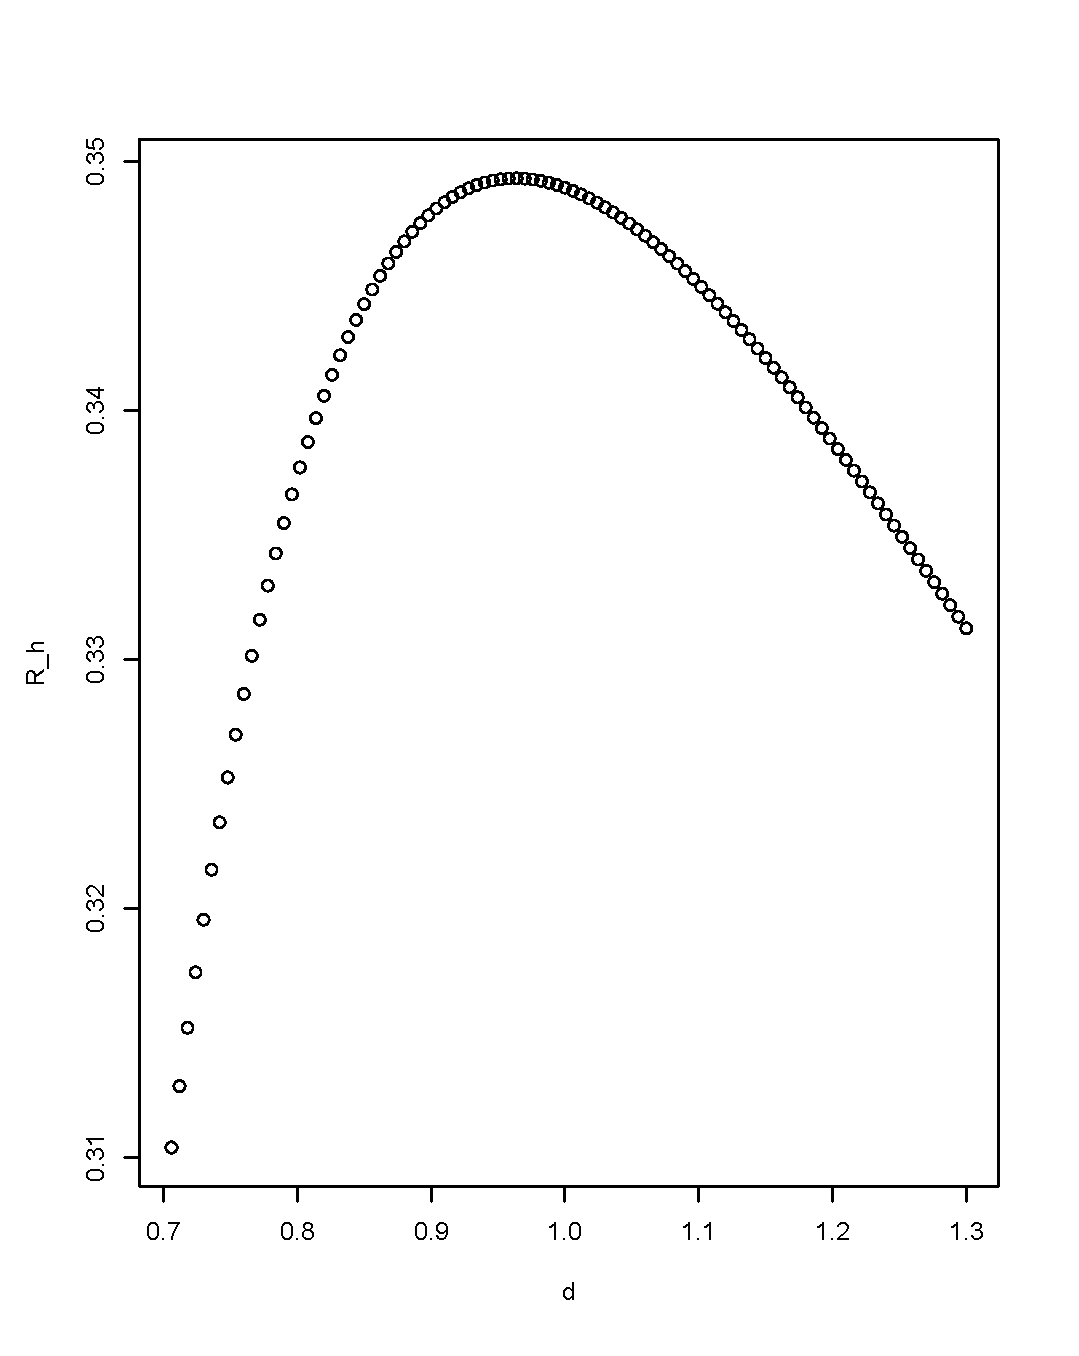
\includegraphics[scale=0.3]{Example2}

\column{0.5\textwidth}
Use software to maximize $R_h$, we have
$$d^*=0.9632226$$
and
$$R_h^*=0.3493290,$$
which is much higher (better) than the best we could achieve with proportional reinsurance.
\end{columns}

\end{frame}
%%%%%%%%%%%%%%%%%%%%%%%%%%%%%%%%%%%%%%%%%%%%%%%%%%%%%%%
\begin{frame}{A Theorem}
If
\begin{itemize}
\item We are in a Cram\'er-Lundberg setting
\item We are considering two reinsurance treaties, one of which is excess of loss
\item Both treaties have same expected payments and same premium loadings
\end{itemize}
then
\begin{itemize}
\item The adjustment coefficient with the excess of loss treaty will always be \alert{at least as good (high) as with any other type of reinsurance treaty}
\end{itemize}

\end{frame}
%%%%%%%%%%%%%%%%%%%%%%%%%%%%%%%%%%%%%%%%%%%%%%%%%%%%%%%

\end{document}